% XCircuit output "BJT_iv_indukc.tex" for LaTeX input from BJT_iv_indukc.ps
\def\putbox#1#2#3#4{\makebox[0in][l]{\makebox[#1][l]{}\raisebox{\baselineskip}[0in][0in]{\raisebox{#2}[0in][0in]{\scalebox{#3}{#4}}}}}
\def\rightbox#1{\makebox[0in][r]{#1}}
\def\centbox#1{\makebox[0in]{#1}}
\def\topbox#1{\raisebox{-0.60\baselineskip}[0in][0in]{#1}}
\def\midbox#1{\raisebox{-0.20\baselineskip}[0in][0in]{#1}}
   \scalebox{0.8}{
   \normalsize
   \parbox{4.36979in}{
   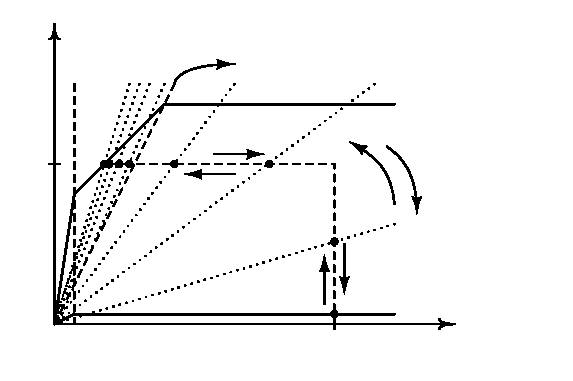
\includegraphics[scale=1.25]{BJT_iv_indukc}\\
   % translate x=287 y=291 scale 0.30
   \putbox{0.06in}{2.50in}{1.20}{$I_C$}%
   \putbox{3.40in}{0.09in}{1.20}{$U_{CE}$}%
   \putbox{1.90in}{2.50in}{1.20}{odpor drift. oblasti}%
   \putbox{3.23in}{2.17in}{1.20}{$I_{B,on}$}%
   \putbox{3.34in}{1.61in}{1.20}{$g_{CE}(t)$}%
   \putbox{1.73in}{1.84in}{1.20}{vyp.}%
   \putbox{1.31in}{1.42in}{1.20}{zap.}%
   \putbox{0.06in}{1.63in}{1.20}{$I_L$}%
   \putbox{2.56in}{0.13in}{1.20}{$U_d$}%
   } % close 'parbox'
   } % close 'scalebox'
   \vspace{-\baselineskip} % this is not necessary, but looks better
